\documentclass[11pt, a4paper]{article}
\usepackage[utf8]{inputenc}
\usepackage[spanish]{babel}
\usepackage{geometry}
\usepackage{graphicx}
\usepackage{listings}
\usepackage{xcolor}

% --- PAQUETE HYPERREF CON LA OPCION PARA QUITAR EL MARCO ---
\usepackage[hidelinks]{hyperref}

% --- Configuracion de margenes ---
\geometry{a4paper, total={170mm,257mm}, left=20mm, top=20mm}

% --- Configuracion para los bloques de codigo ---
\definecolor{codegreen}{rgb}{0,0.6,0}
\definecolor{codegray}{rgb}{0.5,0.5,0.5}
\definecolor{codepurple}{rgb}{0.58,0,0.82}
\definecolor{backcolour}{rgb}{0.95,0.95,0.92}

\lstdefinestyle{mystyle}{
    backgroundcolor=\color{backcolour},   
    commentstyle=\color{codegreen},
    keywordstyle=\color{magenta},
    numberstyle=\tiny\color{codegray},
    stringstyle=\color{codepurple},
    basicstyle=\footnotesize\ttfamily,
    breakatwhitespace=false,         
    breaklines=true,                 
    captionpos=b,                    
    keepspaces=true,                 
    numbers=left,                    
    numbersep=5pt,                  
    showspaces=false,                
    showstringspaces=false,
    showtabs=false,                  
    tabsize=2
}

\lstset{style=mystyle}

% --- Portada ---
\title{Solución de Examen Técnico de Datos}
\author{Alan Alexis Zavala Mendoza}
\date{\today}

% --- Inicio del Documento ---
\begin{document}

\maketitle

\begin{abstract}
El presente documento detalla la solución a un conjunto de problemas de análisis de datos relacionados con el Mercado Eléctrico Mayorista. Se abarca desde la configuración del entorno de trabajo con Docker y PostgreSQL, la creación del esquema de la base de datos, la carga masiva de datos mediante scripts de Python, hasta la resolución de 11 puntos específicos de análisis mediante consultas SQL y la generación de visualizaciones con Python.
\end{abstract}

\tableofcontents

\newpage

% ===================================================================
\section{Configuración del Entorno}
% ===================================================================

\subsection{Base de Datos con Docker}
Para garantizar un entorno de desarrollo reproducible, se utilizó Docker y Docker Compose para levantar un contenedor con una instancia de PostgreSQL.

\subsubsection{Archivo \texttt{docker-compose.yml}}
El siguiente archivo define el servicio de la base de datos, especificando la imagen de PostgreSQL, las credenciales y el volumen para la persistencia de los datos.

\begin{lstlisting}[language=YAML]
# docker-compose.yml
version: '3.8'

services:
  db:
    image: postgres:16-alpine
    container_name: postgres_db
    restart: always
    environment:
      POSTGRES_DB: examen
      POSTGRES_USER: postgres
      POSTGRES_PASSWORD: postgres
    ports:
      - "5432:5432"
    volumes:
      - db_data:/var/lib/postgresql/data

volumes:
  db_data: 
\end{lstlisting}

\subsubsection{Ejecución}
Para levantar el contenedor, se ejecuta el siguiente comando en la terminal desde el directorio donde se encuentra el archivo:
\begin{verbatim}
docker-compose up -d
\end{verbatim}


\subsection{Dependencias de Python}
El análisis de datos y la carga se realizaron con Python. Las librerías necesarias se encuentran en el archivo \texttt{requirements.txt}.
\begin{lstlisting}
# requirements.txt
# pip install -r requirements.txt

simple-salesforce>=1.11.4
pandas>=2.0.3
pyodbc>=4.0.40
pydantic>=2.11.5
python-dotenv>=1.0.0
sqlalchemy>=2.0.41

\end{lstlisting}
Se instalan con el comando: \texttt{pip install -r requirements.txt}

% ===================================================================
\newpage
\section{Creación y Carga de la Base de Datos}
% ===================================================================

\subsection{Creación de Tablas (Schema SQL)}
El esquema de la base de datos fue definido en el archivo \texttt{create\_tables.sql}. Este script se encarga de eliminar las tablas si existen y crearlas con la estructura correcta, incluyendo llaves primarias y columnas auto-incrementales.

\begin{lstlisting}[language=SQL]
CREATE SCHEMA IF NOT EXISTS MemSch;

DROP TABLE IF EXISTS MemSch.MemTraTcDet CASCADE;
CREATE TABLE MemSch.MemTraTcDet (
    idTc INT PRIMARY KEY GENERATED ALWAYS AS IDENTITY,
    fecha DATE NOT NULL,
    valor NUMERIC(10,6),
    FechaUltimaMod TIMESTAMP,
    NombrePcMod VARCHAR(30),
    ClaUsuarioMod INT,
    CONSTRAINT fecha_unica UNIQUE (fecha)
);

DROP TABLE IF EXISTS MemSch.MemTraMDADet CASCADE;
CREATE TABLE MemSch.MemTraMDADet (
    idMDA BIGINT NOT NULL GENERATED ALWAYS AS IDENTITY,
    claNodo VARCHAR(10) NOT NULL,
    fecha DATE NOT NULL,
    hora SMALLINT NOT NULL,
    pml NUMERIC(10,5),
    pml_ene NUMERIC(10,5),
    pml_per NUMERIC(10,5),
    pml_cng NUMERIC(10,5),
    FechaUltimaMod TIMESTAMP,
    NombrePcMod CHAR(30),
    ClaUsuarioMod INT,
    PRIMARY KEY (claNodo, fecha, hora)
);

DROP TABLE IF EXISTS MemSch.MemTraMTRDet CASCADE;
CREATE TABLE MemSch.MemTraMTRDet (
    idMTR BIGINT NOT NULL GENERATED ALWAYS AS IDENTITY,
    claNodo VARCHAR(10) NOT NULL,
    fecha DATE NOT NULL,
    hora SMALLINT NOT NULL,
    pml NUMERIC(10,5),
    pml_ene NUMERIC(10,5),
    pml_per NUMERIC(10,5),
    pml_cng NUMERIC(10,5),
    FechaUltimaMod TIMESTAMP,
    NombrePcMod CHAR(10),
    ClaUsuarioMod INT,
    PRIMARY KEY (claNodo, fecha, hora)
);

DROP TABLE IF EXISTS MemSch.MemTraTBFinVw CASCADE;
CREATE TABLE MemSch.MemTraTBFinVw (
    fecha DATE,
    TbFin NUMERIC(38,14),
    TbFinTGR NUMERIC(38,9)
);
\end{lstlisting}

\newpage
\subsection{Carga de Datos desde CSV}
Se desarrolló un script de Python (\texttt{carga\_csvs.py}) para leer los archivos CSV y cargarlos en las tablas correspondientes de PostgreSQL. El script maneja diferentes formatos de fecha y se asegura de que las columnas coincidan con el esquema de la base de datos.

\begin{lstlisting}[language=Python]
import os
import pandas as pd
from sqlalchemy import create_engine
from sqlalchemy.exc import SQLAlchemyError

def cargar_datos():
    """Carga datos desde archivos CSV a PostgreSQL, asumiendo que las columnas
    de ID son auto-incrementales en la base de datos."""
    db_user = 'postgres'
    db_password = 'postgres'
    db_host = 'localhost'
    db_port = '5432'
    db_name = 'examen'
    schema = 'memsch'
    try:
        engine = create_engine(
            f'postgresql+psycopg2://{db_user}:{db_password}@{db_host}:{db_port}/{db_name}'
        )
        print("Conexion a la base de datos establecida exitosamente.")
    except SQLAlchemyError as e:
        print(f"Error al crear el motor de base de datos: {e}")
        return
    files_to_process = {
        'TC_exa.csv':    {'table': 'memtratcdet',   'format': '%Y-%m-%d'},
        'MDA_exa.csv':   {'table': 'memtramdadet',  'format': '%Y-%m-%d'},
        'MTR_exa.csv':   {'table': 'memtramtrdet',  'format': '%Y-%m-%d'},
        'tbfin_exa.csv': {'table': 'memtratbfinvw', 'format': '%d/%m/%Y'}
    }
    for csv_file, details in files_to_process.items():
        table_name = details['table']
        date_format = details['format']
        file_path = os.path.join(os.getcwd(), csv_file)
        try:
            print(
                f"\nProcesando archivo: '{csv_file}' para la tabla '{schema}.{table_name}'")

            df = pd.read_csv(file_path)
            df.columns = [col.lower() for col in df.columns]

            if 'fecha' in df.columns:
                clean_dates = df['fecha'].astype(str).str.strip()
                df['fecha'] = pd.to_datetime(clean_dates, format=date_format)
            print(f"Cargando {len(df)} registros...")
            df.to_sql(
                name=table_name,
                con=engine,
                schema=schema,
                if_exists='append',
                index=False,
                chunksize=1000
            )
            print(f"Los datos de '{csv_file}' se cargaron en la tabla '{schema}.{table_name}'.")
        except SQLAlchemyError as e:
            print(f"ERROR al procesar el archivo '{csv_file}': {e}")
    print("\n Fin.")
if __name__ == '__main__':
    cargar_datos()
\end{lstlisting}

% ===================================================================
\newpage
\section{Desarollo de requerimientos el examen Python.}
% ===================================================================

Se desarollaron cada uno de los puntos en el Jupyter Notebook anexo, una vez levantado el contenedor con Postgres, creado las tablas y cargado la informacion, el notebook deberia poder ejecutar todas sus secciones sin ningun problema, aqui se detalla el codigo utilizado.

\subsection{Graficar la evolución del precio MDA y MTR del nodo \texttt{01ANS-85}}

Se genero codigo (Notebook) para poder graficar los precios por nodos, filtrando el dataset por el nodo espesificado. 

\begin{lstlisting}[language=Python]
nodo= '01ANS-85'
df_mda = pd.read_sql_table('memtramdadet', engine, schema=schema)
df_mda= df_mda[df_mda['clanodo'] == nodo]
df_mda['datetime'] = pd.to_datetime(df_mda['fecha']) + pd.to_timedelta(df_mda['hora'], unit='h')
df_mtr = pd.read_sql_table('memtramtrdet', engine, schema=schema)
df_mtr = df_mtr[df_mtr['clanodo'] == nodo]
df_mtr['datetime'] = pd.to_datetime(df_mtr['fecha']) + pd.to_timedelta(df_mtr['hora'], unit='h')
plt.style.use('seaborn-v0_8-whitegrid') # Estilo de la gráfica
fig, ax = plt.subplots(figsize=(12, 6)) # Tamaño de la figura
ax.plot(df_mda['datetime'], df_mda['pml'], label=f'PML MDA ({nodo})', marker='o', linestyle='-', markersize=4)
ax.plot(df_mtr['datetime'], df_mtr['pml'], label=f'PML MTR ({nodo})', marker='x', linestyle='--', markersize=4, alpha=0.8)
ax.xaxis.set_major_formatter(mdates.DateFormatter('%Y-%m-%d %H:%M'))
plt.xticks(rotation=45)
ax.set_title(f'Evolución del Precio Marginal Local (PML) para el Nodo {nodo}', fontsize=16)
ax.set_xlabel('Fecha y Hora', fontsize=12)
ax.set_ylabel('PML ($/MWh)', fontsize=12)
ax.legend(fontsize=12)
ax.grid(True, which='both', linestyle='--', linewidth=0.5)
plt.tight_layout()
plt.show()
\end{lstlisting}

Teniendo como resultado la siguiente grafica:
\begin{figure}[h!]
  \centering
  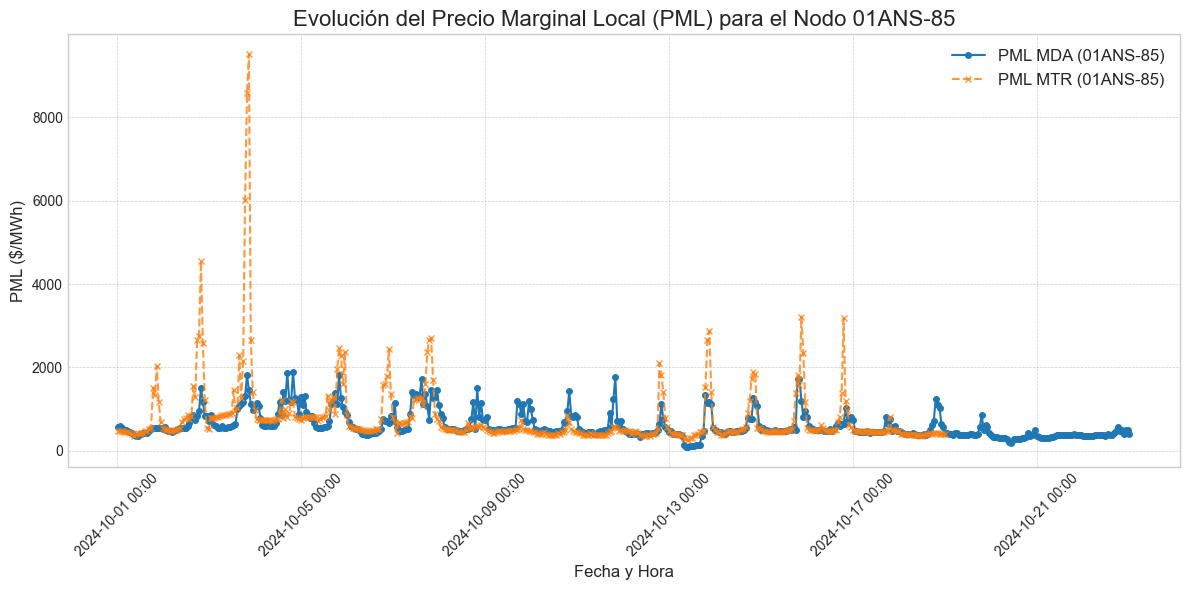
\includegraphics[width=\textwidth,keepaspectratio]{1_gra_ev_mda_mtr_nodo.png}
\end{figure}

\newpage
\subsection{Grafícar la diferencia promedio por día del precio entre el MDA y MTR de todos los nodos agrupados por día.}

Se genero el codigo para graficar la diferencia promedio por dia entrer MDA y MTR, agrupandolos por dia, teniendo el siguiente codigo:

\begin{lstlisting}[language=Python]
df_mda['origen'] = 'MDA'
df_mtr['origen'] = 'MTR'
df_mda_mtr = pd.concat([df_mda, df_mtr], ignore_index=True)
df_mda_mtr['fecha'] = pd.to_datetime(df_mda_mtr['fecha'])
df_diferencia = df_mda_mtr.groupby(['fecha', 'origen'])['pml'].mean().unstack()
df_diferencia['diff_mtr_mda'] = df_diferencia['MTR'] - df_diferencia['MDA']
plt.style.use('seaborn-v0_8-whitegrid')
fig, ax = plt.subplots(figsize=(12, 6))
colores = ['#2ca02c' if x > 0 else '#d62728' for x in df_diferencia['diff_mtr_mda']]
ax.bar(df_diferencia.index, df_diferencia['diff_mtr_mda'], color=colores, width=0.8)
ax.axhline(0, color='black', linewidth=0.8, linestyle='--')
ax.xaxis.set_major_locator(mdates.AutoDateLocator())
ax.xaxis.set_major_formatter(mdates.DateFormatter('%Y-%m-%d'))
plt.xticks(rotation=45)
ax.set_title('Diferencia Promedio Diaria de Precios (PML MTR - PML MDA)', fontsize=16)
ax.set_ylabel('Diferencia de PML ($/MWh)', fontsize=12)
ax.set_xlabel('Fecha', fontsize=12)
ax.grid(True, axis='y', linestyle='--', linewidth=0.5)
plt.tight_layout()
plt.show()
\end{lstlisting}

Obteniendo como resultado la siguiente grafica:
\begin{figure}[h!]
  \centering
  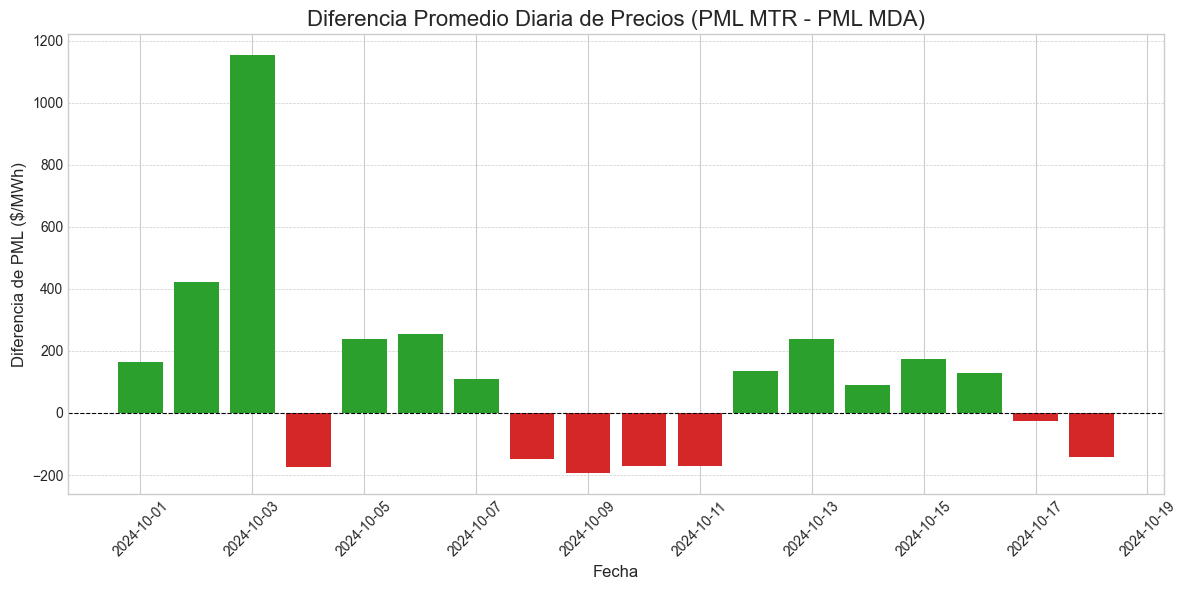
\includegraphics[width=\textwidth,keepaspectratio]{2_diff_prom_precio.png}
\end{figure}

\newpage
\subsection{Une en una sola tabla MemTraMdaDet y MemTraMtrDet agregando una columna al inicio que se llame origen y pueda ser “MDA” o “MTR”.}

\begin{lstlisting}[language=Python]
df_mda = pd.read_sql_table('memtramdadet', engine, schema=schema)
df_mtr = pd.read_sql_table('memtramtrdet', engine, schema=schema)
df_mda['origen'] = 'MDA'
df_mtr['origen'] = 'MTR'
df_mda_mtr = pd.concat([df_mda, df_mtr], ignore_index=True)
df_mda_mtr = df_mda_mtr[['origen'] + df_mda_mtr.columns[df_mda_mtr.columns != 'origen'].tolist()]
df_mda_mtr.head()
\end{lstlisting}



\subsection{Une esta tabla creada en el paso anterior y la de TC, para agregar a una columna de valor para tener tambien el tc}

\begin{lstlisting}[language=Python]
df_tc = pd.read_sql_table('memtratcdet', engine, schema=schema)
df_tc = df_tc[['fecha', 'valor']]
df_tc.rename(columns={'valor': 'tipo_cambio'}, inplace=True)
df_mda_mtr_tc = pd.merge(df_mda_mtr, df_tc, on='fecha', how='left')
df_mda_mtr_tc.head()
\end{lstlisting}

\subsection{Genera un DataFrame Nodo,fecha,hora,pml,tbfin de los datos que el pml sea mayor que la tbfin}

\begin{lstlisting}[language=Python]
df_mda = pd.read_sql_table('memtramdadet', engine, schema=schema)
df_mtr = pd.read_sql_table('memtramtrdet', engine, schema=schema)
df_tbfin = pd.read_sql_table('memtratbfinvw', engine, schema=schema)
df_mda_mtr = pd.concat([df_mda, df_mtr], ignore_index=True)
df_mda_mtr['fecha'] = pd.to_datetime(df_mda_mtr['fecha'])
df_tbfin['fecha'] = pd.to_datetime(df_tbfin['fecha'])
df_mda_mtr_tbfin = pd.merge(df_mda_mtr, df_tbfin, on='fecha', how='left')
df_pml_hi_tbfin = df_mda_mtr_tbfin[df_mda_mtr_tbfin['pml'] > df_mda_mtr_tbfin['tbfin']][['clanodo', 'fecha', 'hora', 'pml', 'tbfin']]
df_pml_hi_tbfin.head()
\end{lstlisting}

\subsection{Genera un dataframe que tenga el promedio diario de los precios del pml}

\begin{lstlisting}[language=Python]
df_mda = pd.read_sql_table('memtramdadet', engine, schema=schema)
df_mtr = pd.read_sql_table('memtramtrdet', engine, schema=schema)
df_precios = pd.concat([df_mda, df_mtr], ignore_index=True)
df_promedio_diario = df_precios.groupby('fecha')['pml'].mean().reset_index()
df_promedio_diario.rename(columns={'pml': 'pml_promedio_diario'}, inplace=True)
df_promedio_diario.head()
\end{lstlisting}

\newpage
\subsection{Grafica el precio del Nodo y el precio de la tbfin por fecha y hora}

Se genero el codigo para graficar el precio del nodo y precio de la tbfin, utilizando el siguiente codigo:

\begin{lstlisting}[language=Python]
df_mda = pd.read_sql_table('memtramdadet', engine, schema=schema)
df_mtr = pd.read_sql_table('memtramtrdet', engine, schema=schema)
df_tbfin = pd.read_sql_table('memtratbfinvw', engine, schema=schema)
df_precios = pd.concat([df_mda, df_mtr], ignore_index=True)
df_precios['fecha'] = pd.to_datetime(df_precios['fecha'])
df_tbfin['fecha'] = pd.to_datetime(df_tbfin['fecha'])
nodo_a_analizar = '01ANS-85'
df_nodo = df_precios[df_precios['clanodo'] == nodo_a_analizar].copy()
df_nodo['datetime'] = pd.to_datetime(df_nodo['fecha']) + pd.to_timedelta(df_nodo['hora'], unit='h')
df_final = pd.merge(df_nodo, df_tbfin[['fecha', 'tbfin']], on='fecha', how='left')
df_final.sort_values('datetime', inplace=True)
plt.style.use('seaborn-v0_8-whitegrid')
fig, ax = plt.subplots(figsize=(12, 6))
ax.plot(df_final['datetime'], df_final['pml'], label=f'PML Nodo {nodo_a_analizar}', color='royalblue', zorder=2)
ax.plot(df_final['datetime'], df_final['tbfin'], label='TBFin (Diario)', color='darkorange', linestyle='--', linewidth=2, zorder=3)
ax.xaxis.set_major_formatter(mdates.DateFormatter('%Y-%m-%d %H:%M'))
plt.xticks(rotation=45)
ax.set_title(f'Comparativa de Precios: Nodo {nodo_a_analizar} vs. TBFin', fontsize=16)
ax.set_xlabel('Fecha y Hora', fontsize=12)
ax.set_ylabel('Precio ($/MWh)', fontsize=12)
ax.legend(fontsize=12)
ax.grid(True, which='both', linestyle='--', linewidth=0.5)
plt.tight_layout()
plt.show()
\end{lstlisting}

Obteniendo como resultado la siguiente grafica:
\begin{figure}[h!]
  \centering
  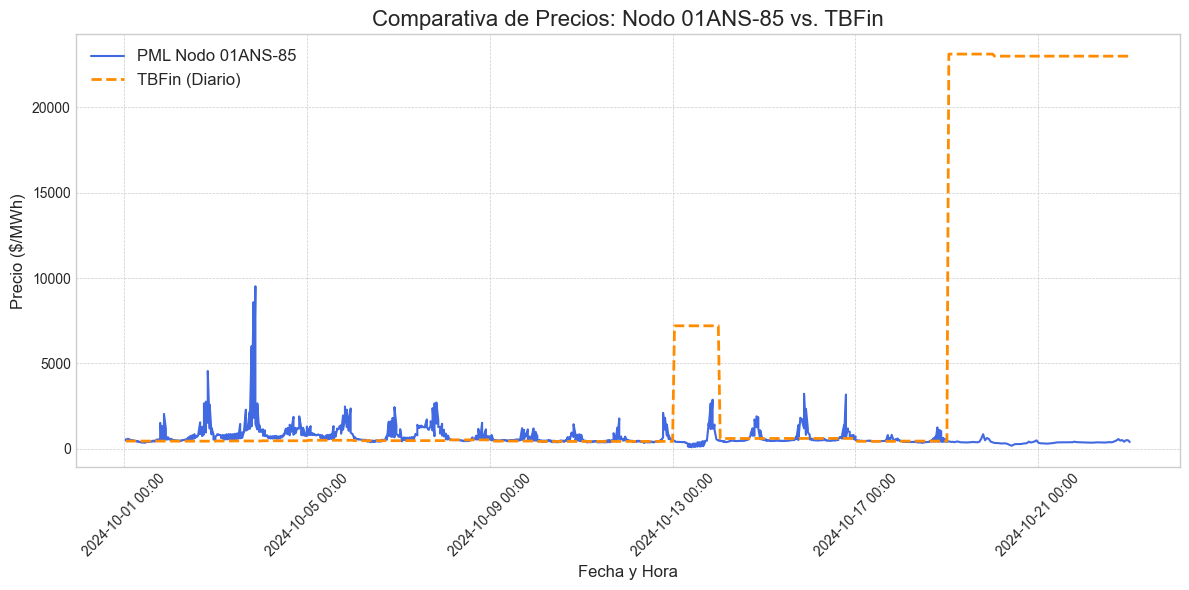
\includegraphics[width=\textwidth,keepaspectratio]{3_comp_precios.png}
\end{figure}

% ===================================================================
\newpage
\section{Desarollo de requerimientos el examen SQL.}
% ===================================================================

A continuación se proporcionan las queries necesarias para cubrir los puntos 8 a 11 del examen. De la misma manera, se incluyen en el \texttt{Notebook} para su ejecución y visualización, así como en el archivo SQL (\texttt{examen\_seccion\_sql.sql}) anexo.

\subsection{Query que me traiga el precio del nodo (pml) en MDA y el precio en MTR del nodo 01ANS-85, ordenado por nodo (ascendente) , por fecha (descente) y ascendente por hora.}

\begin{lstlisting}[language=SQL]
SELECT
    COALESCE(mda.claNodo, mtr.claNodo) AS claNodo,
    COALESCE(mda.fecha, mtr.fecha) AS fecha,
    COALESCE(mda.hora, mtr.hora) AS hora,
    mda.pml AS pml_mda,
    mtr.pml AS pml_mtr
FROM
    MemSch.MemTraMDADet AS mda
FULL OUTER JOIN
    MemSch.MemTraMTRDet AS mtr ON mda.claNodo = mtr.claNodo
                               AND mda.fecha = mtr.fecha
                               AND mda.hora = mtr.hora
WHERE
    COALESCE(mda.claNodo, mtr.claNodo) = '01ANS-85'
ORDER BY
    claNodo ASC,
    fecha DESC,
    hora ASC;
\end{lstlisting}

\subsection{Query que me traiga el precio promedio por nodo en MTR y en MDA, y la diferencia de estos 2 precios promedio, ordenado por diferencia descendentemente.}

\begin{lstlisting}[language=SQL]
WITH mda_promedio AS (
    SELECT
        claNodo,
        AVG(pml) AS pml_promedio_mda
    FROM
        MemSch.MemTraMDADet
    GROUP BY
        claNodo
),
mtr_promedio AS (
    SELECT
        claNodo,
        AVG(pml) AS pml_promedio_mtr
    FROM
        MemSch.MemTraMTRDet
    GROUP BY
        claNodo
)
SELECT
    COALESCE(mda.claNodo, mtr.claNodo) AS nodo,
    mda.pml_promedio_mda,
    mtr.pml_promedio_mtr,
    (mtr.pml_promedio_mtr - mda.pml_promedio_mda) AS diff_mda_mtr
FROM
    mda_promedio AS mda
FULL OUTER JOIN
    mtr_promedio AS mtr ON mda.claNodo = mtr.claNodo
ORDER BY
    diff_mda_mtr DESC;
\end{lstlisting}

\newpage
\subsection{Proporciona el precio de nodo en dlls tomando como tipo de cambio el campo valor que esta en la tabla MEMTraTcDet}

\begin{lstlisting}[language=SQL]
WITH precios AS (
    SELECT claNodo, fecha, hora, pml FROM MemSch.MemTraMDADet
    UNION ALL
    SELECT claNodo, fecha, hora, pml FROM MemSch.MemTraMTRDet
)
SELECT
    p.claNodo,
    p.fecha,
    p.hora,
    p.pml,
    tc.valor AS tipo_de_cambio,
    (p.pml * tc.valor) AS pml_en_dolares
FROM
    precios AS p
INNER JOIN
    MemSch.MemTraTcDet AS tc ON p.fecha = tc.fecha
ORDER BY
    p.fecha,
    p.claNodo,
    p.hora;
\end{lstlisting}

\subsection{Proporciona el listado de nodos por fecha, hora, de los precios de los nodos en mda y mtr, junto con el tipo de cambio y el precio de la tbfin}

\begin{lstlisting}[language=SQL]
WITH precios AS (
    SELECT
        COALESCE(mda.claNodo, mtr.claNodo) AS claNodo,
        COALESCE(mda.fecha, mtr.fecha) AS fecha,
        COALESCE(mda.hora, mtr.hora) AS hora,
        mda.pml AS pml_mda,
        mtr.pml AS pml_mtr
    FROM
        MemSch.MemTraMDADet AS mda
    FULL OUTER JOIN
        MemSch.MemTraMTRDet AS mtr ON mda.claNodo = mtr.claNodo
                                   AND mda.fecha = mtr.fecha
                                   AND mda.hora = mtr.hora
)
SELECT
    p.claNodo,
    p.fecha,
    p.hora,
    p.pml_mda,
    p.pml_mtr,
    tc.valor AS tipo_de_cambio,
    tb.tbfin
FROM
    precios AS p
LEFT JOIN
    MemSch.MemTraTcDet AS tc ON p.fecha = tc.fecha
LEFT JOIN
    MemSch.MemTraTBFinVw AS tb ON p.fecha = tb.fecha
ORDER BY
    p.fecha,
    p.claNodo,
    p.hora;
\end{lstlisting}

\end{document}